\begin{figure}[tp]
\footnotesize
\centering
	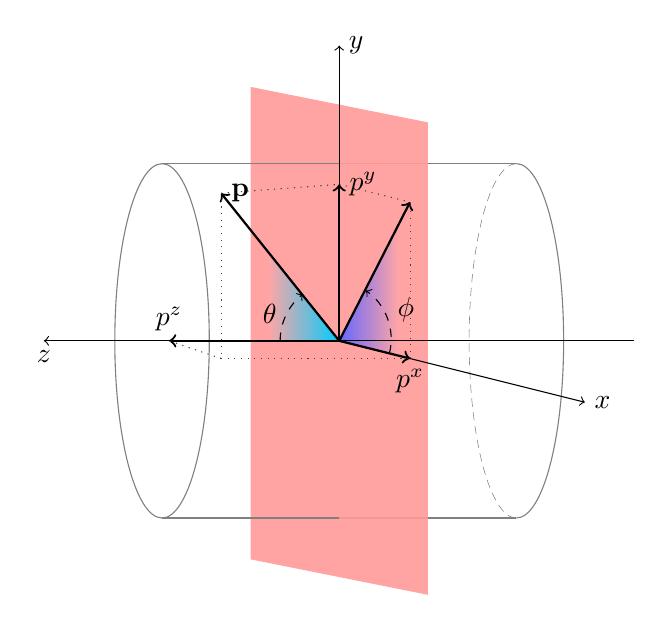
\begin{tikzpicture}[scale=0.75]
	
		\draw[gray] (-2.2,0) arc[x radius = 0.8, y radius = 3, start angle= 0, end angle= 360];
		\draw[gray] (3,3) -- (0,3); \draw[gray] (3,-3) -- (0,-3);
		\draw[gray,very thin,densely dashed] (3,3) arc[x radius = 0.8, y radius = 3, start angle= 90, end angle= 270];
		
		\draw[draw=none,fill=red!40!white,opacity=.9] (-1.5,4.3)--(1.5,3.7)--(1.5,-4.3)--(-1.5,-3.7)--cycle;

		\draw[gray] (3,-3) arc[x radius = 0.8, y radius = 3, start angle= -90, end angle= 90];
  	 	
  	 	\draw[gray] (0,3) -- (-3,3); \draw[gray] (0,-3) -- (-3,-3);
  	 	
  	 	
  	 	\draw[draw=none,  left color= blue!60!white, right color=red!35!white] (0,0)--(1,-0.25) -- (1,1.95) --cycle;
  	 	\draw[draw=none, right color= cyan!80!blue, left color=red!35!white] (0,0)--(-1.2,0) -- ( -1.2,1.53) --cycle;
  	 	\draw[->,dashed] (-1,0) arc [radius=1, start angle=180, end angle= 128] node[left =12pt, below]{$\theta$};
  	 	\draw[->,dashed] (0.85,-0.2125) arc [radius=1, start angle=-14.04, end angle= 55.3] node[below=7pt, right=8pt]{$\phi$};
  	 	
  	 	\draw[->,thick] (0,0)--(-2,2.5) node [right] {$\textbf{p}$};
  	 	\draw[->,thick] (0,0)--(1.2,2.35) node [right] {\textbf{\pt}};
  	 	\draw[->,thick] (0,0)--(-2.88,0) node [above ] {$p^{z}$};
  	 	\draw[->,thick] (0,0)--(1.2,-0.3) node [below ] {$p^{x}$};
  	 	\draw[->,thick] (0,0)--(0,2.65) node [right ] {$p^{y}$};
  	 	
  	 	\draw[thin,dotted,darkgray] (-2,2.5)--(-2,-0.3);
		\draw[thin,dotted,darkgray] (-2,-0.3)--(1.2,-0.3);
		\draw[thin,dotted,darkgray] (1.2,-0.3)--(1.2,2.35);
		\draw[thin,dotted,darkgray] (-2,2.5)--(0,2.65);
		\draw[thin,dotted,darkgray] (0,2.65)--(1.2,2.35);
		\draw[thin,dotted,darkgray] (-2,-0.3)--(-2.88,0);
		

		%===ASSI===
		\draw [->,thin] (5,0)--(-5,0) node[below]{$z$};
		\draw [->,thin] (0,0)--(4.16,-1.04) node[right]{$x$};
		\draw [->,thin] (0,0)--(0,5) node[right]{$y$};
	
	\end{tikzpicture}
	\caption{Sketch of the frame of reference used in the ATLAS detector which is represented as a simple cilinder. The $z$ axis points along the beam, the $y$ axis points upwars and the $x$ axis points toward the center of LHC ring. The polar angle $\theta$ and the azimuthal angle $\phi$ are represented. The vector $\textbf{p}$ is decomposed in its component $(p^x,p^y,p^z)$ and its transverse part $\textbf{\pt}=p^x \textbf{e}_x+p^y \textbf{e}_y$ lying in the red transverse plane in the middle is pointed out.}
\label{fig:coordinate}
\end{figure}